\section{Constraint Satisfaction Problems}
\begin{itemize}
	\item Knowledge Representation is focused on qualitative reasoning, not really quantitative
	\begin{itemize}
		\item Abstract description of the world is mostly easier for human to reason than an exact numerical definition 
		\item We can for example reason about time points and intervals in our system where we have relations between those
	\end{itemize}
\end{itemize}
\subsection{Fundamentals of CSPs}
\begin{itemize}
	\item To represent qualitative knowledge, we again have to define a:
	\begin{itemize}
		\item \textit{Vocabulary}: finite set of relations, mostly binary. 
		
		Example: $x$ equals $y$ $\Rightarrow$ $x=y$, $x$ before $y$ $\Rightarrow$  $x<y$, $x$ after $y$ $\Rightarrow$  $x>y$
		\item \textit{Language}: sets of atomic formulae, perhaps restricted disjunction
		
		Example: define disjunction by $x\left\{<,=\right\}y$ (in maths $x\leq y$), and formulae to describe configurations: $\left\{x\left\{<,=\right\}y, y\left\{z\right\}\right\}$
		\item \textit{Formal semantics}: interpretation of function and symbols
		
		Example: interpret time points and relations over rational (or real) numbers
	\end{itemize}
	\item On those, we can perform various reasoning tasks
	\begin{itemize}
		\item \textit{Satisfiability}: Is this a consistent set of constraints? $\Rightarrow$ find satisfying instantiation of all variables
		\item \textit{Deduction}: Does $x\left\{=\right\}y$ logically follow from the configuration?
		\item \textit{Minimal description}: What are the most constrained relations that describe the same set? 
		\item \textit{Solving}: find one or all (optimal) solutions to the CSP
	\end{itemize}
	\item Formally, a Constraint Satisfaction Problem consists of:
	\begin{itemize}
		\item Variables $Y:=y_1, y_2, ..., y_k$
		\item Domains $D_1, ..., D_k$ to which the variables belong ($y_i$ represents a possible value of $D_i$: $y_i\in D_i$)
		\item Constraints $C\in \mathcal{C}$ on $Y$ which define a subset of $D_1 \times D_2 \times ... \times D_k$ 
	\end{itemize}
	\item Given a CSP $\left\{\mathcal{C}; y_1\in D_1, ..., y_k\in D_k \right\}$, $\left(d_1, ..., d_k\right)\in D_1\times ...\times D_k$ is a solution iff for all $C\in \mathcal{C}: \left(d_1, ..., d_k\right)\in C$
	\item Most CSPs have only binary constraints (constraints over two variables) which can be modeled by a constraint graph (nodes are variables, edges/arcs are constraints)
\end{itemize}
\subsubsection{Backtrack search}
\begin{itemize}
	\item Finding a solution for CSPs is a more general version of DPLL (PL is actually a special case CSP)
	\item In the initial state, we have an empty set of assignments. We then assign a value to an unassigned variable that does not conflict with the current assignment. Test if CSP is fulfilled or unsatisfied for this assignment. If neither of both, choose the next variable etc.
	\item The depth of the search tree is the number of variables, and the number of children/splits in the tree are given by the domain size. In the worst case, we have a search space of $|D|^{\# vars}$
	\item We can improve backtracking efficiency by:
	\begin{enumerate}
		\item \textbf{Smart variable picking}: various heuristics for choosing the next variable
		\begin{itemize}
			\item \textit{Most constrained variable}: choose the variable with the fewest legal values (therefore also called \textit{Minimum remaining values} (MRV))
			\item \textit{Most constraining variable}: the variable with the most constraints on. Is mostly used as tie-breaker strategy for MRV
		\end{itemize}
		\item \textbf{Smart value picking}: what possible value of the domain to pick for the variable
		\begin{itemize}
			\item \textit{Least constraining value}: given a variable, choose the value that constraints the least, i.e. the one that rules out the fewest values in the remaining values  
		\end{itemize}
		\item \textbf{Spotting failure early} to backtrack early: finding unsatisfiable constraints in a branch
		\begin{itemize}
			\item \textit{Forward checking}: by keeping track of remaining legal values for unassigned variables, we can stop the search in this branch if one variable has an empty set/no legal values to be assigned. This is done by propagating information from assigned to unassigned variables.
			\item \textit{Arc consistency}: simplest form of constraint propagation (see Section~\ref{sec:constraint_propagation}) that makes each arc/edge consistent. Hence, $x\to y$ is consistent iff for every value $x$ in $D_x$ there exists a value $y$ in $D_y$ for which the constraint is satisfied (if not, remove contradicting values of $D_x$). Note that if $x$ has been changed, we have to recheck all its neighbors. Arc consistency can detect failures earlier than forward checking
			\item More complex/sophisticated methods are discussed under constraint propagation in Section~\ref{sec:constraint_propagation}
		\end{itemize}
	\end{enumerate}   
\end{itemize}
\subsection{Constraint propagation}
\label{sec:constraint_propagation}
\begin{itemize}
	\item A constraint itself can restrict the search space without splitting
	\item Constraint propagation is similar to unit propagation and subsumes resolution. It therefore checks the CSP for local consistency (a CSP is locally consistent if we can extend it by another assignment while being satisfied)
	\item Example: the CSP $\langle x < y ; x \in \left[50..200\right], y \in \left[0..100\right] \rangle$ can be simplified to 
	
	$\langle x < y ; x \in \left[50..99\right], y \in \left[51..100\right] \rangle$ without losing any possible solutions
	\item This might be an iterative problem when multiple constraints interact with each other ($x$ has effect on $y$, $y$ on $z$, and so on)
	\item Thus, we have to decide when to stop performing local consistency checking. There are various heuristics/methods:
	\begin{itemize}
		\item \textit{(Directional) Arc consistency} is one of the most simplest approaches. Note that general arc consistency applies propagation to both sides $x\to y$ and $y\to x$, while we can also limit it by a directed approach (only $x\to y$ or $y\to x$). Problem: only looks at direct constraints and can for example not spot that the following CSP is inconsistent:
		
		\begin{figure}[ht!]
			\centering
			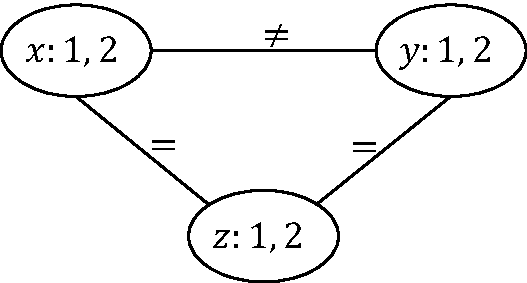
\includegraphics[width=0.3\textwidth]{figures/kr_csp_arc_const_example.pdf}
		\end{figure}
		\item \textit{Path consistency}: extends arc consistency to picking two variables. Formally, for all $i$ and $j$:
		$$\forall x,y: (x,y)\in P_{i,j}, x\in P_i, y\in P_j \to \left(\exists z: z \in P_k \wedge (x,z) \in P_{i,k} \wedge (z,y) \in P_{k,j}\right)$$
		i.e., any consistent assignment to two variables can be extended to a third one. Can be enforced by iterating the following assignment until nothing changes anymore:
		$$P_{i,j} := P_{i,j} \cap \left\{(x,y)\hspace{1mm}|\hspace{1mm}\exists z: (x,z) \in P_{i,k} \wedge (z,y) \in P_{k,j}\hspace{2mm}\text{for all } k\right\}$$
		Path consistency subsumes arc consistency and detects inconsistency in the previous example. Note that path consistency removes pairs of values, and thus makes constraints explicitly
		\item \textit{$k$-Consistency}: generalization of arc and path consistency to arbitrary $k$. For each satisfying value assignment to $k-1$ variables, there exists an extension of this assignment to a $k$-th variable such that this extended assignment satisfies all constraints among these $k$ variables.
		\item \textit{Strong $k$-consistency}: A CSP is strongly $k$-consistent iff it is $j$-consistent for all $j\leq k$. If a CSP of size $n$ $n$-consistent is, then we can construct a model in polynomial time. But note that checking this already solves the CSP and the computational costs exponentially grow with $k$.
		\item \textcolor{red}{Question: why does PC subsumes AC, but not $k$-consistency $k-1$-consistency?}
		\item \textit{Hyper-arc consistency}: extension of arc consistency to more than binary constraints (same for those). Defined by: for every constraint $C$ and every variable $x$ with domain $D_x$, each value for $x$ from $D_x$ participates in a solution to $C$.
	\end{itemize}
\end{itemize}